
%(BEGIN_QUESTION)
% Copyright 2006, Tony R. Kuphaldt, released under the Creative Commons Attribution License (v 1.0)
% This means you may do almost anything with this work of mine, so long as you give me proper credit

{\it Flame ionization detectors}, often referred to as {\it FID}s, exploit the principle of electrical conductivity in a flame to detect the presence of trace substances in a hydrogen gas stream.  FIDs are often used as detectors on industrial gas chromatographs, especially in the petrochemical industries where most compounds of interest contain carbon.

Hydrogen, when burned, does not create ions in the flame.  However, quantities of hydrocarbon compounds mixed with hydrogen gas will generate ions in the flame, which may then be detected electrically.  The strength of the electrical signal will be in proportion to the concentration of carbon atoms mixed in the hydrogen gas stream.

A simplified FID is shown here, the ``exhaust'' gases from the burner passing through a hollow metal ring acting as a ``collector'' for ions generated in the flame:

$$\includegraphics[width=15.5cm]{i00657x01.eps}$$

Explain how the operational amplifier in this circuit works to convert the small ionic current into an output voltage.  Also, determine whether the resistor in the feedback loop of the opamp circuit should be of a large, small, or modest resistance value.

\vskip 20pt \vbox{\hrule \hbox{\strut \vrule{} {\bf Suggestions for Socratic discussion} \vrule} \hrule}

\begin{itemize}
\item{} Describe how an FID placed at the tail-end of a gas chromatograph column will respond as a complex hydrocarbon sample passes through the column.
\item{} Explain why a flame ionization detector may be classified as an {\it amperometric} sensor, as opposed to a {\it potentiometric} sensor such as a pH glass electrode.
\item{} Identify a fault in this system that could cause the output of this detector to always be zero (i.e. indicate no ions when in fact there are ionizable species in the sample).
\end{itemize}

\underbar{file i00657}
%(END_QUESTION)





%(BEGIN_ANSWER)

Current carried by the flame is pulled through the resistor by the opamp's negative feedback action, thus producing a measurable voltage at the output of the opamp.  The more carbon in the flame, the more current, and the more voltage output by the opamp.  

\vskip 10pt

Since the amount of current through the flame is exceedingly small, the resistor needs to be very large in order to develop a respectable amount of voltage.

%(END_ANSWER)





%(BEGIN_NOTES)


%INDEX% Chemistry, ionization: in a flame
%INDEX% Measurement, analytical: carbon (in a gas)

%(END_NOTES)


